\subsection{Data description}
The training data $imgs$ contains 8545 color images of size 105x43. From every image a HOG descriptor 26x10x36 was extracted and converted into a vector of total length 9360. All of these descriptors make up the training data on which we will work on.  We noticed that there are more images without people (7308 negative samples) than with people (1237 positive samples).

\noindent Our task is to train various classifiers, so that we will be able to detect the presence of people in new images. For this purpose we evaluate five classifiers, measuring the accuracy of their estimations using Receiver Operating Characteristics (ROC) curves.

\subsection{Data preprocessing}
\noindent We assume that there are no outliers, since the images are manually annotated. We work on the extracted features so we normalize the 9360 dim vectors to have  0 mean and standard deviation 1. For all the methods presented below we used 5 fold cross validation.

The methods that we compare are: Naive Bayes classifier, Logistic and Penalized Logistic Regresion, Support Vector Machine (SVM),  K-NN, and Neural Network classifier. 
We note that before the experiments we tried using PCA for reducing the dimensionality of the feature descriptors. The reduction in dimensionality was minimal but at a huge computational cost so we decided to drop it.
\subsection{Naive Bayes classifier}
\noindent In this part we tried to fit a Naive Bayes classifier to our data. For this, we made the assumption that the data is normally distributed and the estimates of the prior probabilities can be estimated empirically from the relative frequencies of the classes in training samples.

The results from the K-fold validation were not very satisfying, since the average TPR was very low (0.031). This may be caused by the strong assumptions that we made in order to fit this model. Naive Bayes model assumes that the processed data follows a specific distribution (in our case Gaussian), but also that the features are independent. In our data, this is possibly not the case, so the classifier cannot fit an appropriate model.
\subsection{Logistic and Penalized Logistic Regression}
\noindent Our goal in this part was to train a simple Logistic Regression model and its Penalized version as baseline methods. We chose a learning parameter $\alpha = 10^{-2}$, since all the values close to this performed well enough for our experiments. Regarding the value  $\lambda$ for penalized logistic regression, all of the values that were used performed the same.  Both of the methods gave the same results, with average TPR equal to 0.754.

 By adding a penalization term, we tried to prevent overfitting by imposing penalty on large fluctuations of the model parameters and reduce the influence of the outliers to our model. The data, as we mentioned before, does not have outliers and the fluctuations at the model parameters are avoided by the nature of our data. This is possibly the reason that both models performed similarly. 
\subsection{Support Vector Machines}
\noindent For this part of the experiments we used the LIBSVM 3.20\footnote{http://www.csie.ntu.edu.tw/~cjlin/libsvm/} toolbox that supports SVM with various kernels.  We performed analysis and K-fold validation on linear-kernel SVM, polynomial-kernel SVM with degrees 2 and 3, radial-basis-function SVM and sigmoid-kernel SVM. In all the models we used the prediction scores to compute the TPR and the FPR. A comparison of the various model is given in Fig \ref{fig:SVM}.

We observe that the RBF SVM performs significantly better. This fact can be seen not only by looking at the average TPR, equal to 0.893, but also oberving the whole range of the FPR, where the classifier gives better results than all of the other SVM models. The second best in performance is polynomial SVM with degree 2, which has very similar results with the RBF case for FPR greater than $10e{-3}$. The rest of the classifiers perform well for FPR greater than $10e{-2}$, with the exception of the linear case, which has quite good results for lower rates, too.  Cubic SVM performed worse than Quadratic SVM probably due to overfitting on the training data. We also present in Table \ref{table:SVM_success} the average percentage of the successful classifications that were made during the K-fold validation:
\begin{table}[h]
  \centering
  \begin{tabular}{ | c | c | c | c | c | c |}
  \hline
  SVM kernel & Linear & Quadratic & Cubic & RBF & Sigmoid \\ \hline
  Average success rate (\%) & 94.81 & 97.22 & 91.45 & 98.43 & 84.68 \\ \hline
  \end{tabular}
  \captionof{table}{Average percentage for the success rate of SVM classifiers.}
  \label{table:SVM_success}
\end{table}
\subsection{K-NN classifier}
\noindent For this experiments we used a KNN library, which we modified in order to compute and return as output not only the class labels, but also the scores of the prediction.
We used Euclidean Distance as distance measure between samples and varied the number of neighbours between 5, 9, 15, 19, 25. 

\noindent Fig \ref{fig:K_NN} presents the resulting ROC curves that were created using the scores obtained from the K-fold validation runs. All the classifiers show good performance, especially for FPR greater than $10^{-3}$. Only the 9-NN classifier seems to perform a bit worse for FPR between $10^{-4}$ and $10^{-3}$. For FPR greater than  $10^{-3}$
the algorithms perform similarly, resulting in almost overlapping curves.

\begin{figure}[h]
  \centering
  \begin{subfigure}[b]{0.49\textwidth}
   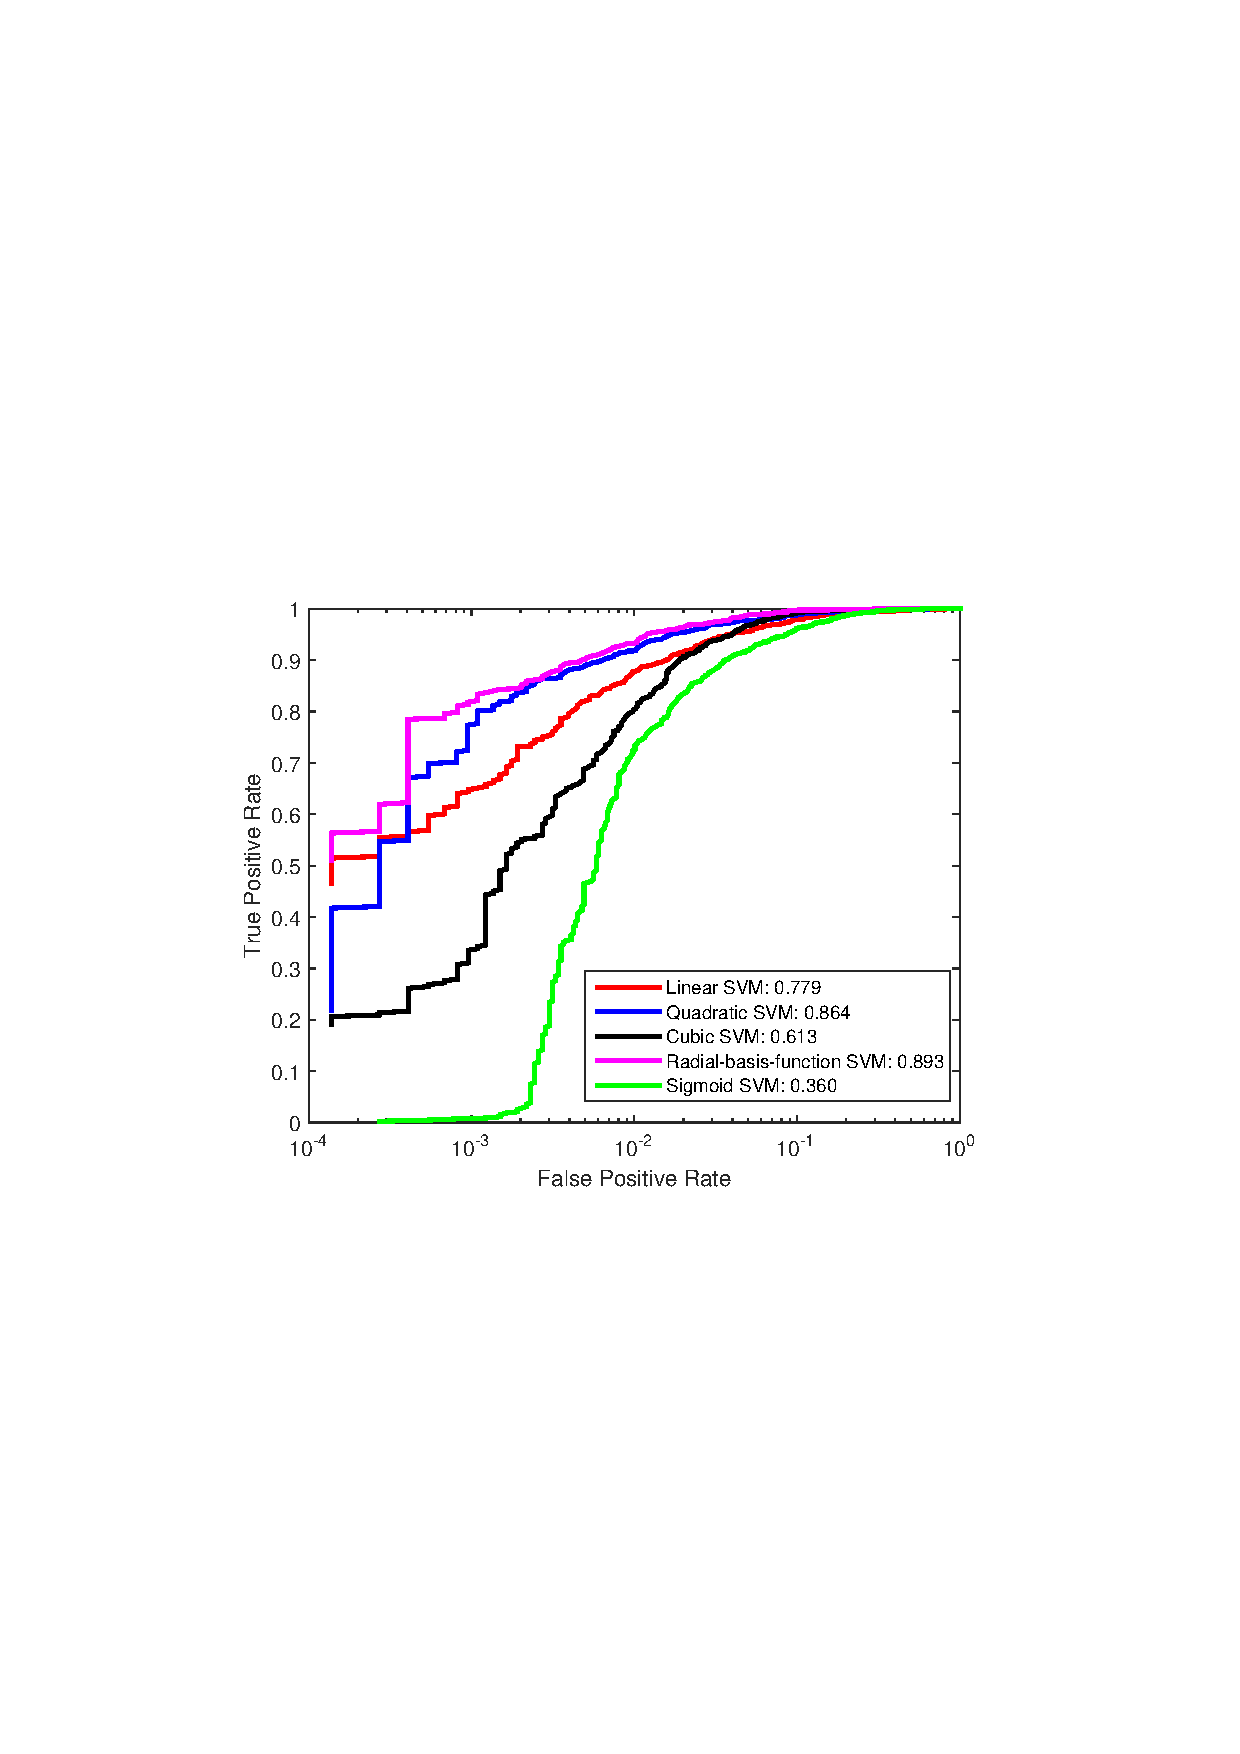
\includegraphics[width=\textwidth]{figures/SVM.pdf}
    \caption{}
    \label{fig:SVM}
  \end{subfigure}
  \begin{subfigure}[b]{0.49\textwidth}
    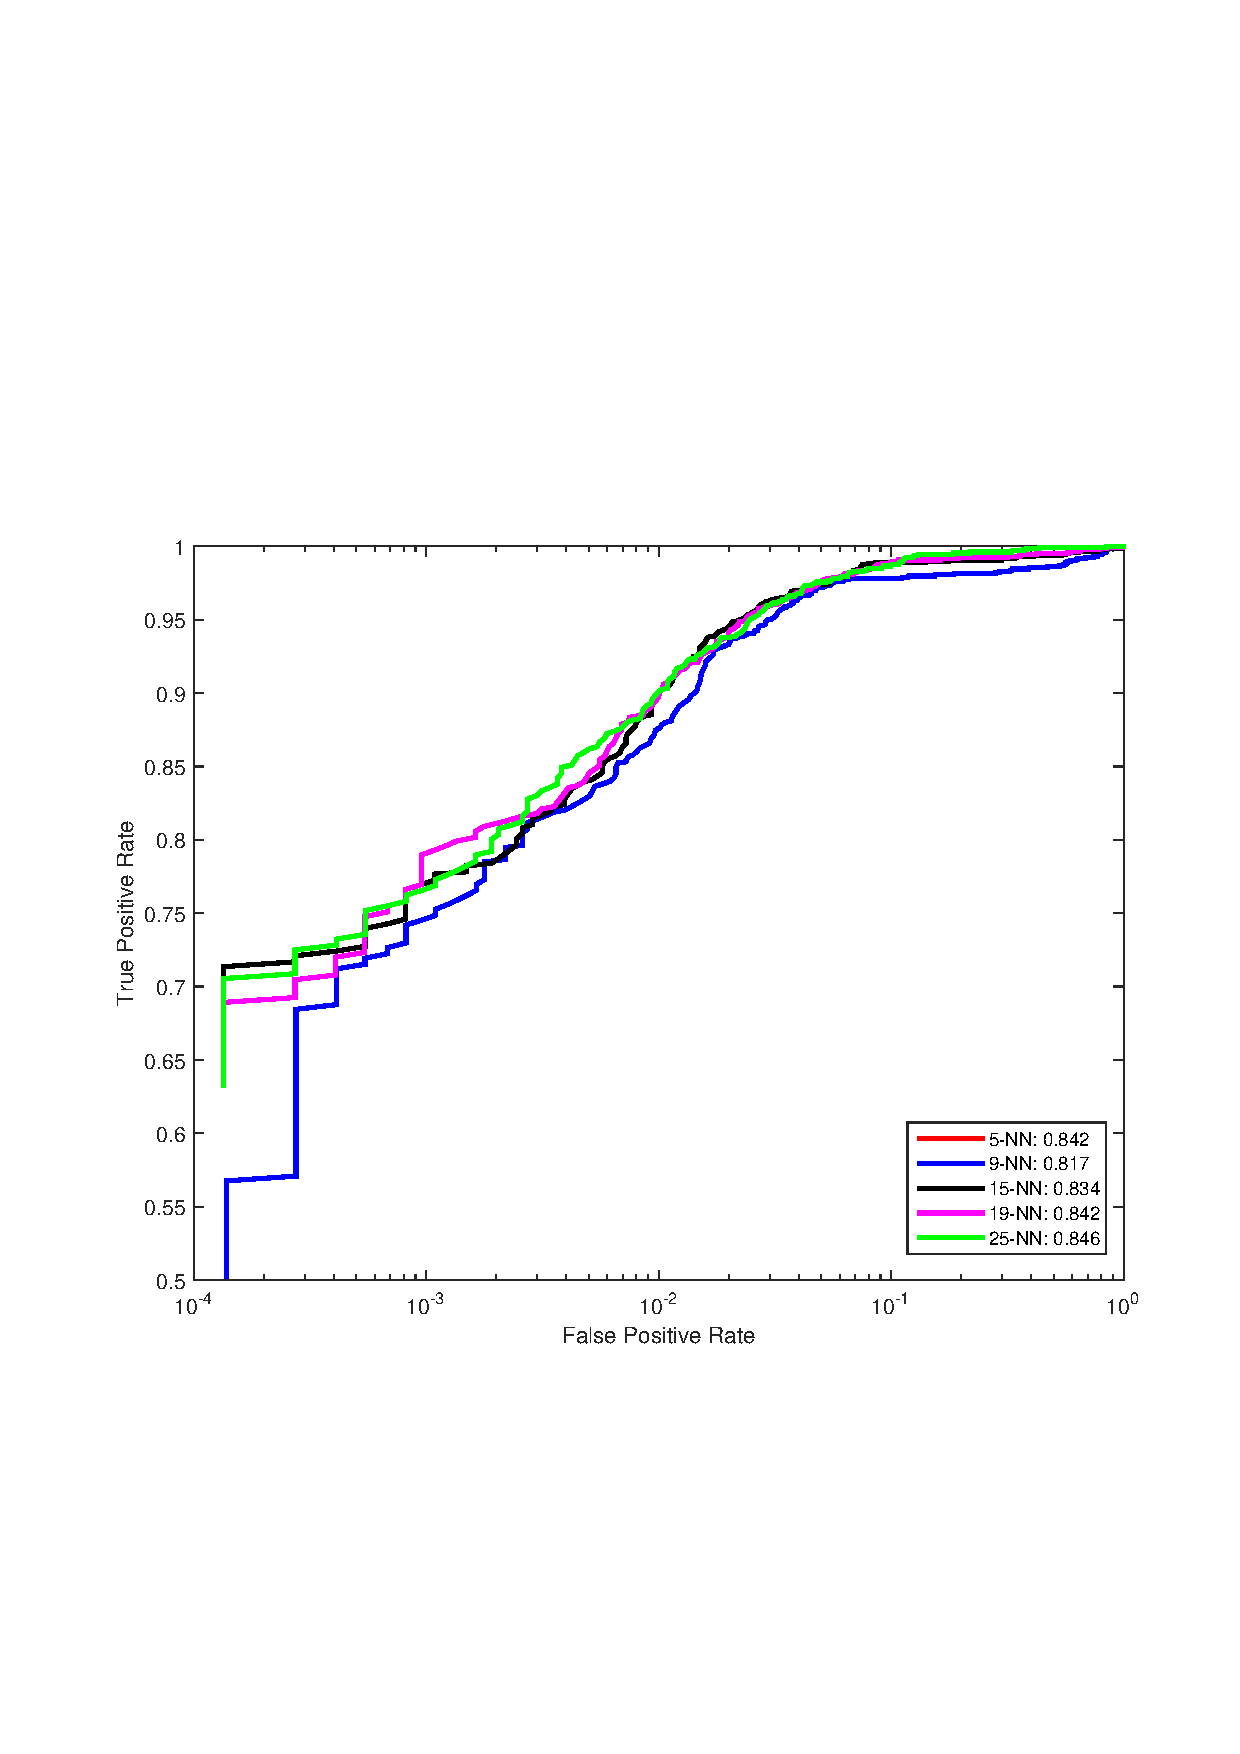
\includegraphics[width=\textwidth]{figures/K_NN.pdf}
    \caption{}
    \label{fig:K_NN}
  \end{subfigure}
  \caption{ROC curves created using: (a) SVM with various kernel types (linear, quadratic, cubic, real-basis-function, sigmoid), (b) K-NN classifier for various number of neighbours (5, 9, 15, 19, 25).}
\end{figure}
\subsection{Neural Network}
Neural Networks are powerfull tools able to learn complex decisions boundaries. Besides the computational cost, their major drawback is the high amount of parameters needed to be tuned for a specific problem, making them harder to train.

The parameters we considered for our problem were the number of epochs, the learning rate $\alpha$ (parameter in gradient descent update), the number of hidden layers and their size. We fixed the batch size to 50 and the number of epochs to 10, since we experimentally saw that the error starts to converge after 10 passes through the data. The activation functions were also kept fixed to tanh (hyperbolic tangent) for intermediate layers and sigmoid at the last layer. 

Using cross validation for a network with just one hidden layer of 50 neurons we determined the learning parameter $\alpha$, which we later used for bigger network setups. Fig.\ref{fig:NNa}  shows the ROC curves for $\alpha$ in  $[0.01,0.1,1,10]$.

The results for bigger setups can be seen in Fig \ref{fig:NNb}. Choosing $\alpha=1$, we experimented with 2 hidden layers of sizes $[50,20],[100,50],[200,50],[200,100]$ and $[300,50]$. The smallest NN performed just slightly worse than the others for FPR less than $10^{-3}$, meaning we  can increase a bit the model complexity by adding more neurons per layer or more hidden layers.  We could have easily increased and test larger networks if it were not for the time and computational contraints. Not suprisingly, our best setup consists in the biggest network. We see that increasing the size of the network leads to smaller FPR in the range $10^{-4}$ -$10^{-2}$ and better performance in general. However, the improvements are rather small compared to the increased complexity that was added.

\begin{figure}[h]
  \centering
  \begin{subfigure}[b]{0.49\textwidth}
   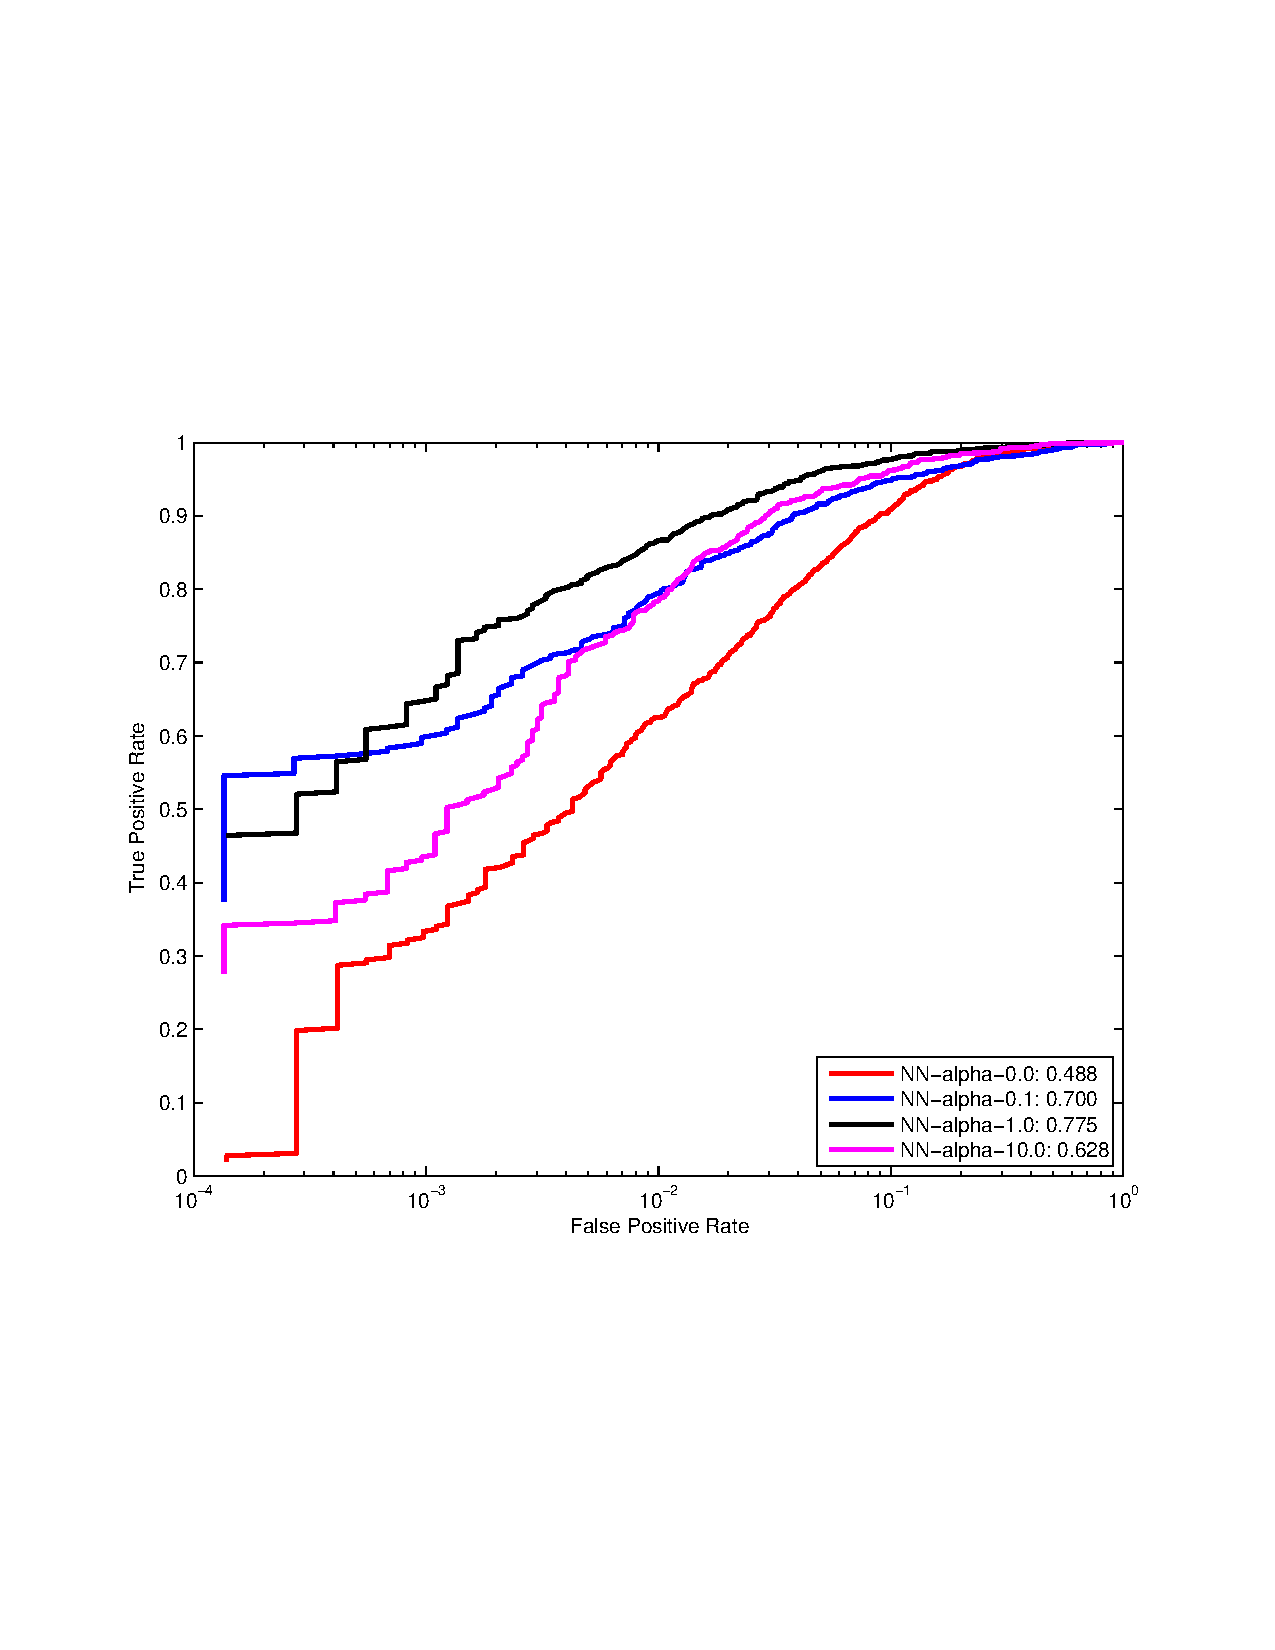
\includegraphics[width=\textwidth]{figures/NN-alpha.pdf}
    \caption{}
    \label{fig:NNa}
  \end{subfigure}
  \begin{subfigure}[b]{0.49\textwidth}
    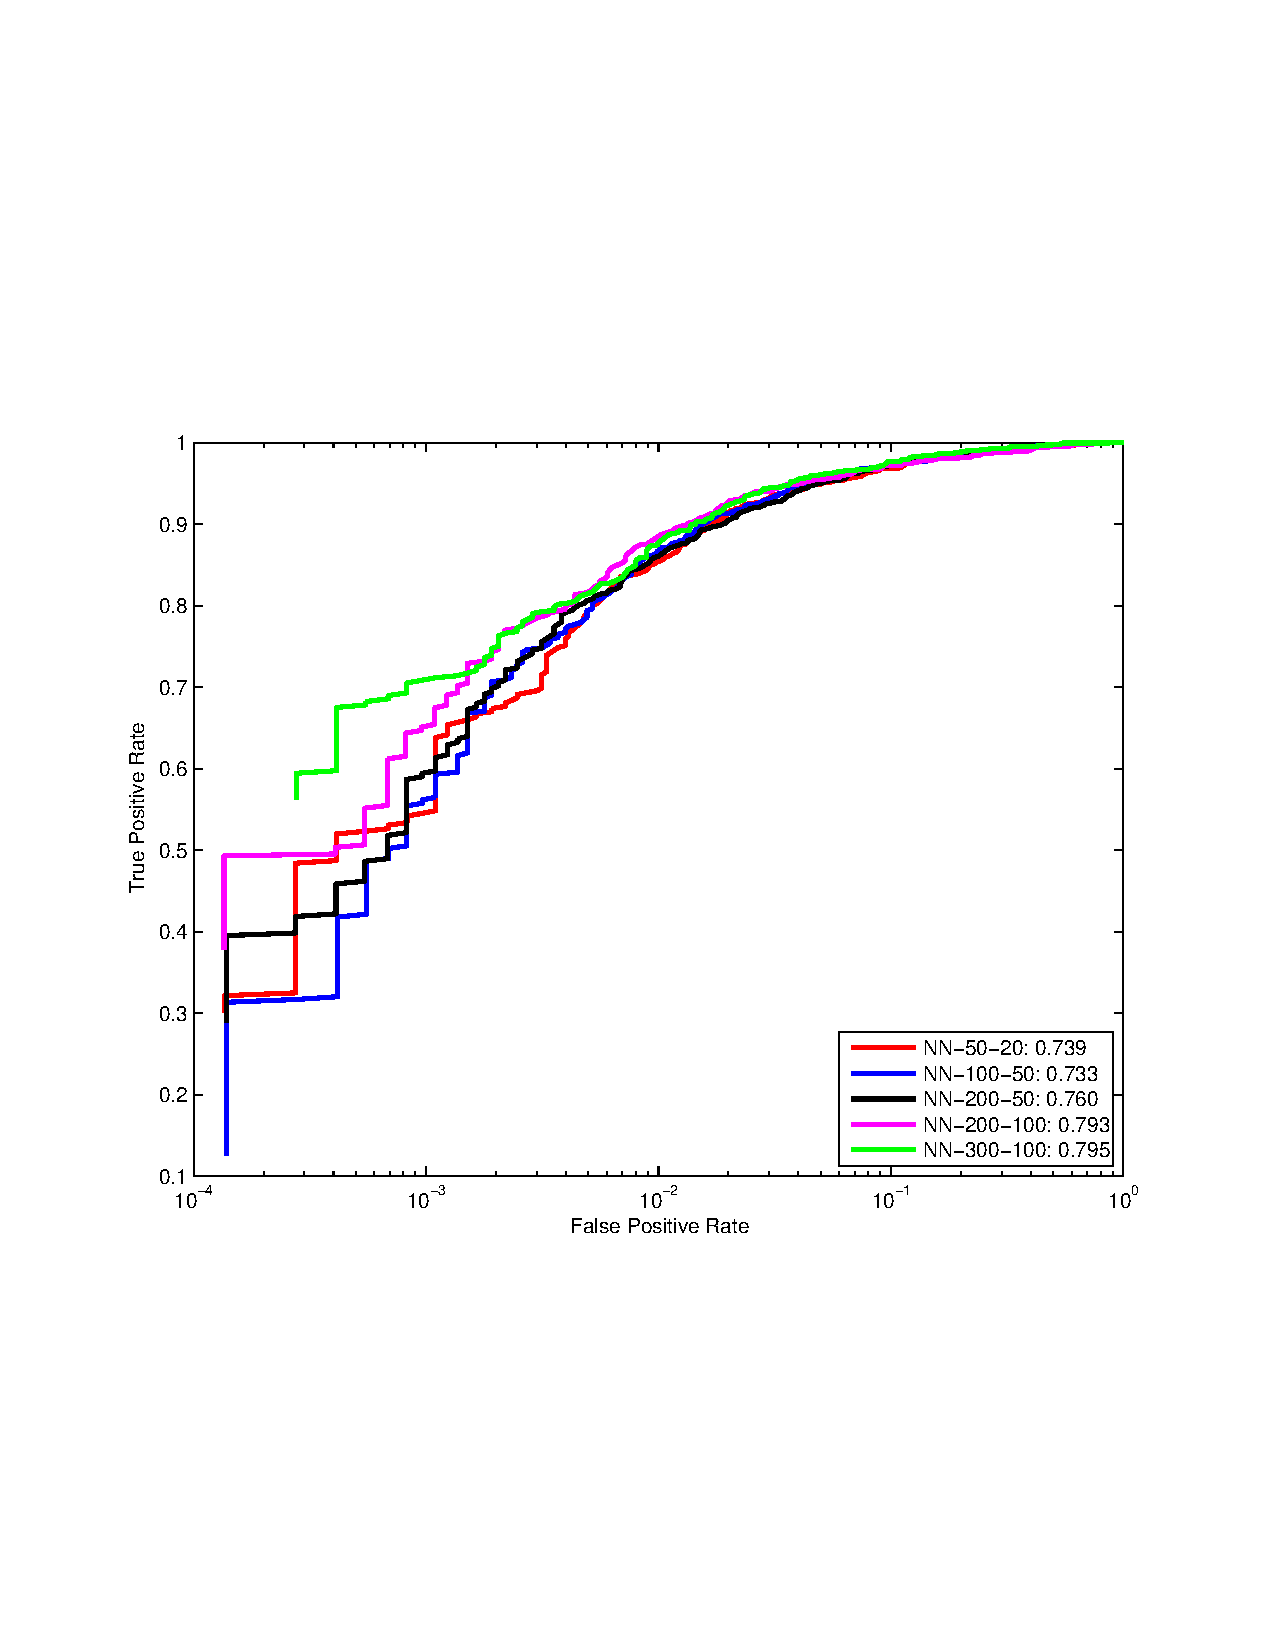
\includegraphics[width=\textwidth]{figures/NN-2layers.pdf}
    \caption{}
    \label{fig:NNb}
  \end{subfigure}
  \caption{ROC curves created using: (a) NN with one hidden layer of 50 neurons, $\alpha$ in $[0.01,0.1,1,10]$ (b) NN with two layers of various sizes. In the legend, NN-50-20 corresponds to a network of 50 and respectively 20  neurons for the 1st and 2nd hidden layer.}
\end{figure}

\subsection{Comparison}
To sum up, the models that performed best on the people detection data were SVM (with RBF or Quadratic kernels) followed closely by KNN with 25 neighbours and Euclidean Distance as metric. Although our NN setups performed just a little better than Penalized Logistic Regression, we believe different setups (e.g. 3 intemediate layers or different activation functions) would have fitted better. 
We note that our models depend on the discriminative power of the HOG features. Using the same models but with different feature descriptors would have changed the rankings of our best models. 
